Las oscilaciones son paralelas a la dirección del movimiento de la onda. En otras palabras, la dirección del movimiento de las oscilaciones y el de la onda ocurre en el mismo eje.

Dada la naturaleza de la vibración perpendicular del campo eléctrico y magnético, este tipo de onda no puede ser \electromagnetica.

\begin{figure}[H]
  \centering
  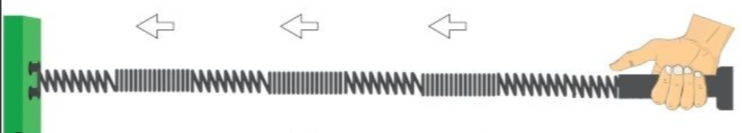
\includegraphics[scale=0.4]{imagenes/onda_longitudinal.png}
  \caption{Onda longitudinal\cite{educacao}}
\end{figure}

Este tipo de onda presenta partes de \textbf{compresión} y \textbf{expansión}.

La \textbf{compresión} ocurre cuando hay alta frecuencia, por tanto cada oscilación está más cerca de las otras. Esto da la impresión de que la onda está comprimida.

La \textbf{expansión} ocurre cuando hay baja frecuencia, por tanto cada oscilación está más lejos de las otras. Esto da la impresión de que la onda está dilatada.

Ejemplos:

\begin{itemize}
  \item Ondas sonoras.
  \item Ondas en un resorte.
  \item Ondas sísmicas.
\end{itemize}
